% 电动力学

\pentry{经典力学\upref{CM0}}

本科阶段通常会有几门不同深度关于电磁场场的课程, 第一门往往叫做\textbf{电磁学(electromagnetism)}, 比较高级的课程叫做\textbf{电动力学(electrodynamics)}. 从课程内容上来说, 电磁学就是简单的电动力学. 严格来说, 电动力学强调场和电荷的运动规律, 如果研究静止的电荷和电磁场, 可以将其称为\textbf{静电学(electrostatics)}或\textbf{静磁学(magnetostatics)}. 我们以下统一使用电动力学.

经典力学研究若干粒子(质点)受若干力后的运动情况,这里的粒子可以是任何有质量的粒子,力也可以是任何力.电动力学研究的是一堆带电荷的质点(既有质量又有电荷)受一堆电磁力后的运动情况.所以唯一需要做的是,弄清如何计算这些电磁力,再用经典力学就可以得出粒子的运动.

\subsection{电磁力和电磁场}

\begin{figure}[ht]
\centering
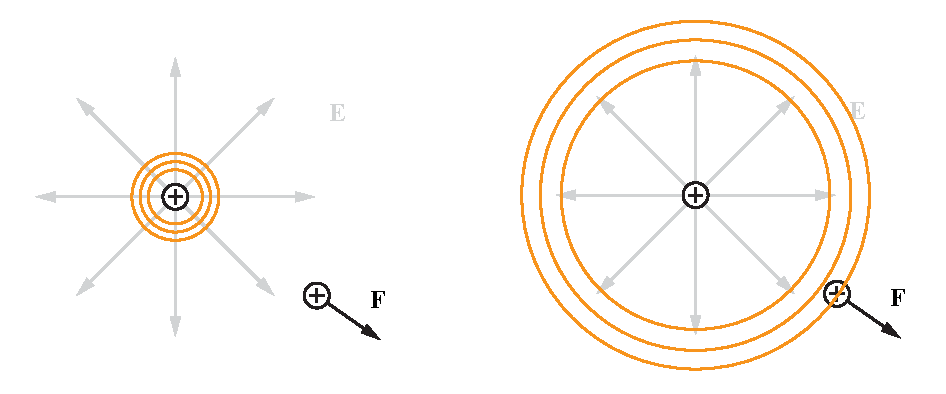
\includegraphics[width=14cm]{./figures/EM01.pdf}
\caption{静止的电荷突然振动几下又停下来,扰动就会以电磁波(橙色部分)的形式向外传播,到达另一电荷的位置时,才会有力的变化.图中只画出了一个电荷产生的场.} \label{EM0_fig1}
\end{figure}

经典力学中万有引力是超距的,就是说只要两个质点存在,不管他们相隔多远都会立即有作用力(与质量和距离有关),如果它们之间的距离发生改变,那么这个作用力也会立即改变.这是不合理的(现在我们知道任何信息的传递都不可能超过光速,如果一个粒子动一下,另一个粒子马上就能感到力的变化,那就可以超过光速传递信息).电动力学不同,我们需要先计算电场和磁场(场就像波一样,传播需要时间),再根据粒子所在位置的场计算粒子的受力(其他地方的场如何与粒子受力无关).例如库仑定理的形式虽然和万有引力一样,但是在电动力学中我们先计算一个粒子在另一个粒子处产生的电场,再计算处于该电场中的粒子所受电场力(库仑力).当两个粒子都静止时,这么做似乎和直接由距离计算力有没有区别,但如果某时刻其中一个粒子抖动了一下,电场(先不提磁场)就会像扰动的水波一样将这个扰动沿各个方向以一定的速度传播,直到传播到另一个粒子所在的地方,另一个粒子才能从电场中感觉到受力的变化.

磁场虽然产生的方式和对粒子的作用与电场不同,但也会像波一样传播.事实上,电场和磁场并不是独立传播的,上面说的电场扰动的传播时必须同时借助磁场.

\subsection{电荷}
电荷在电动力学中扮演了两个角色.一是电磁场是由电荷产生的.二是只有带电荷的粒子在电磁场中才会受力,其他粒子不会.

\subsection{麦克斯韦方程组}
麦克斯韦方程组是一组写描述场变化规律的数学公式.可以想象成一个懂电动力学的计算机,只要告诉它所有的带电粒子在哪里,以及如何运动(位置关于时间的函数),它就能计算出空间中任何一点的电磁场.和机械波(如水波)不同,电场和磁场在每个位置都既有方向也有大小(有方向和大小的量叫做矢量,这种场叫做矢量场).

麦克斯韦方程组是电动力学的公设之一.

\subsection{电磁力}
任何一个带电粒子某时刻受到的电磁力(也叫广义洛伦兹力),都可以由它所在的位置处的电磁场(两个矢量)以及它当时运动速度(也是矢量)通过公式计算出来.这是电动力学的另一个公设.

可见,在经典力学的基础上加上麦克斯韦方程和广义洛伦兹力的公式后,如果我们知道一堆带电粒子在某个时刻的运动状态(位置和速度),我们就可以知道接下来每个粒子如何运动.
